%% beamer/knitr slides 
%% for Statistical Modeling and Data Visualization course @ UMass
%% Nicholas Reich: nick [at] schoolph.umass.edu


\documentclass[table]{beamer}\usepackage[]{graphicx}\usepackage[]{color}
% maxwidth is the original width if it is less than linewidth
% otherwise use linewidth (to make sure the graphics do not exceed the margin)
\makeatletter
\def\maxwidth{ %
  \ifdim\Gin@nat@width>\linewidth
    \linewidth
  \else
    \Gin@nat@width
  \fi
}
\makeatother

\definecolor{fgcolor}{rgb}{0.345, 0.345, 0.345}
\newcommand{\hlnum}[1]{\textcolor[rgb]{0.686,0.059,0.569}{#1}}%
\newcommand{\hlstr}[1]{\textcolor[rgb]{0.192,0.494,0.8}{#1}}%
\newcommand{\hlcom}[1]{\textcolor[rgb]{0.678,0.584,0.686}{\textit{#1}}}%
\newcommand{\hlopt}[1]{\textcolor[rgb]{0,0,0}{#1}}%
\newcommand{\hlstd}[1]{\textcolor[rgb]{0.345,0.345,0.345}{#1}}%
\newcommand{\hlkwa}[1]{\textcolor[rgb]{0.161,0.373,0.58}{\textbf{#1}}}%
\newcommand{\hlkwb}[1]{\textcolor[rgb]{0.69,0.353,0.396}{#1}}%
\newcommand{\hlkwc}[1]{\textcolor[rgb]{0.333,0.667,0.333}{#1}}%
\newcommand{\hlkwd}[1]{\textcolor[rgb]{0.737,0.353,0.396}{\textbf{#1}}}%
\let\hlipl\hlkwb

\usepackage{framed}
\makeatletter
\newenvironment{kframe}{%
 \def\at@end@of@kframe{}%
 \ifinner\ifhmode%
  \def\at@end@of@kframe{\end{minipage}}%
  \begin{minipage}{\columnwidth}%
 \fi\fi%
 \def\FrameCommand##1{\hskip\@totalleftmargin \hskip-\fboxsep
 \colorbox{shadecolor}{##1}\hskip-\fboxsep
     % There is no \\@totalrightmargin, so:
     \hskip-\linewidth \hskip-\@totalleftmargin \hskip\columnwidth}%
 \MakeFramed {\advance\hsize-\width
   \@totalleftmargin\z@ \linewidth\hsize
   \@setminipage}}%
 {\par\unskip\endMakeFramed%
 \at@end@of@kframe}
\makeatother

\definecolor{shadecolor}{rgb}{.97, .97, .97}
\definecolor{messagecolor}{rgb}{0, 0, 0}
\definecolor{warningcolor}{rgb}{1, 0, 1}
\definecolor{errorcolor}{rgb}{1, 0, 0}
\newenvironment{knitrout}{}{} % an empty environment to be redefined in TeX

\usepackage{alltt}


%       ************************************************
%       **        LaTeX preamble to be used with all 
%	**        statsTeachR labs/handouts.
%
%	Author: Nicholas G Reich
%	Last modified: 14 January 2014
%	************************************************

% \documentclass[table]{beamer}

%	Set theme (a nice plain one)
\usetheme{Malmoe}

%	Use named colors, set main color of theme
%		to match Web site color:
\definecolor{MainColor}{RGB}{10, 74, 109}
\colorlet{MainColorMedium}{MainColor!50}
\colorlet{MainColorLight}{MainColor!20}
\usecolortheme[named=MainColor]{structure} 

%	For tables
%[dvipsnames] [table]
\usepackage{xcolor}

%% calling tabu.sty, assuming a particular directory structure
\usepackage{../../slide-includes/tabu}	% Even fancier than tabulary
\usepackage{multirow}

%	Just for the degree symbol
\usepackage{textcomp}

%	Get rid of footline (page, author, etc. on each slide)
\setbeamertemplate{footline}{}
%	Get rid of navigation buttons
\setbeamertemplate{navigation symbols}{}

%	Make footnotes not ugly
\usepackage{hanging}
\setbeamertemplate{footnote}{\raggedright\hangpara{1em}{1}\makebox[1em][l]{\insertfootnotemark}\footnotesize\insertfootnotetext\par}

%	Text style for code snippets inline in text:
\newcommand{\codeInline}[1]{\texttt{#1}}

%	Text style for emphasis stronger than \emph:
%		(Note, this doesn't toggle the way \emph does.
%			(Note, this can be done, didn't seem worth the trouble.))
\newcommand{\strong}[1]{{\bfseries{#1}}}


%        ******	Define title page	**********************
\setbeamertemplate{title page}{
	{\color{MainColor}
	% There must be a better way than this -vspace at
	%	 the top and bottom of the page to reduce the 
	%	 bottom margin, but I can't find one that works.
	\vspace{-6em}

% 	% Go to a lot of trouble to get the title in a
% 	%	nice box, since customizing a beamer block
% 	%	does not entirely work here (I don't know why)
	\newlength{\titleBoxWidth}
	\setlength{\titleBoxWidth}{\textwidth}
	\addtolength{\titleBoxWidth}{-2.0em}
	\setlength{\fboxsep}{1.0em}
	\setlength{\fboxrule}{0pt}
	\fcolorbox{MainColor!25}{MainColor!25}{
		\parbox{\titleBoxWidth}{
			\raggedright
			\LARGE\textbf{\inserttitle}
		}	% end parbox
	}	% end fcolorbox

	\vfill
	\small{Author: \insertauthor}
	\vspace{\baselineskip}

	\small{\Course}

	\small{\Instructor}
	\vspace{\baselineskip}

	%\small{\emph{This material is part of the \strong{statsTeachR} project}}

	\vspace{0.33\baselineskip}\scriptsize{\emph{\LicenseText}}


		\vspace{-15em}

	}	% end color
	\clearpage
}	% end define title page

%	The following variables are assumed by the standard preamble:
%	Global variable containing module name:
\title{Visual perception in data graphics}
%	Global variable containing module shortname:
%		(Currently unused, may be used in future.)
\newcommand{\ModuleShortname}{introRegression}
%	Global variable containing author name:
\author{Nicholas G Reich}
%	Global variable containing text of license terms:
\newcommand{\LicenseText}{Made available under the Creative Commons Attribution-ShareAlike 3.0 Unported License: http://creativecommons.org/licenses/by-sa/3.0/deed.en\textunderscore US }
%	Instructor: optional, can leave blank.
%		Recommended format: {Instructor: Jane Doe}
\newcommand{\Instructor}{}
%	Course: optional, can leave blank.
%		Recommended format: {Course: Biostatistics 101}
\newcommand{\Course}{}


\input{../../slide-includes/shortcuts}

\hypersetup{colorlinks,linkcolor=,urlcolor=MainColor}


%	******	Document body begins here	**********************
\IfFileExists{upquote.sty}{\usepackage{upquote}}{}
\begin{document}

%	Title page
\begin{frame}[plain]
	\titlepage
\end{frame}

%	******	Everything through the above line must be placed at
%		the top of any TeX file using the statsTeachR standard
%		beamer preamble. 




%%%%%%%%%%%%%%%%%%%%%%%%%%%%%%%%%%%%%%%%%%

\begin{frame}[fragile]{Visual cues}
\begin{block}{Graphical elements that draw attention}

The choice of which visual cues you use inform the story that you are able to convey and the points you can highlight. 

\vspace{3em}

We will go through a set of visual cues. These are loosely adapted from Nathan Yau via the Modern Data Science with R textbook.

\end{block}

% \begin{table}
% \begin{center}
% \begin{tabular}{cccc}
% cue & variable & question & How used \\
% position & numerical & Where in relation to other things? & Points, axis alignment \\
% length & numerical & How big (in one dimension)? & Bars, lines \\
% angle & numerical & How wide? Parallel to something else?  & Lines, pie charts, ...\\
% \end{tabular}
% \end{center}
% \end{table}%

\end{frame}

%%%%%%%%%%%%%%%%%%%%%%%%%%%%%%%%%%%%%%%%%%

\begin{frame}[fragile]{Visual cues: position (numerical)}

\begin{block}{Where are the data in relation to each other?}

e.g. points and axis alignment.
\end{block}

\vspace{15em}

\end{frame}

%%%%%%%%%%%%%%%%%%%%%%%%%%%%%%%%%%%%%%%%%%

\begin{frame}[fragile]{Visual cues: Length (numerical)}

\begin{block}{How big (in one dimension)?}

e.g. bars, lines (aligned), lines(unaligned) ...

\end{block}

\vspace{15em}

\end{frame}


%%%%%%%%%%%%%%%%%%%%%%%%%%%%%%%%%%%%%%%%%%

\begin{frame}[fragile]{Visual cues: Angle (numerical)}

\begin{block}{How wide? Parallel to something else?}

e.g. lines, pie wedges, ...

\end{block}

\vspace{15em}

\end{frame}

%%%%%%%%%%%%%%%%%%%%%%%%%%%%%%%%%%%%%%%%%%

\begin{frame}[fragile]{Visual cues: Direction/slope (numerical)}

\begin{block}{Up or down? At what slope?}

e.g. lines, time-series, ...

\end{block}

\vspace{15em}

\end{frame}

%%%%%%%%%%%%%%%%%%%%%%%%%%%%%%%%%%%%%%%%%%

\begin{frame}[fragile]{Visual cues: Shape (categorical)}

\begin{block}{Belonging to which group?}

e.g. points

\end{block}

\vspace{15em}

\end{frame}

%%%%%%%%%%%%%%%%%%%%%%%%%%%%%%%%%%%%%%%%%%

\begin{frame}[fragile]{Visual cues: Area/volume (numerical)}

\begin{block}{How big (in 2/3 dimensions)?}

e.g. circles, squares

\end{block}

\vspace{15em}

\end{frame}


%%%%%%%%%%%%%%%%%%%%%%%%%%%%%%%%%%%%%%%%%%

\begin{frame}[fragile]{Visual cues: Shade/intensity (categorical or numerical)}

\begin{block}{To what extent? How severely?}

e.g. points, lines, ...

\end{block}

\vspace{15em}

\end{frame}

%%%%%%%%%%%%%%%%%%%%%%%%%%%%%%%%%%%%%%%%%%

\begin{frame}[fragile]{Visual cues: Color  (categorical or numerical)}

\begin{block}{Belonging to which group? To what extent? How severely?}

e.g. points, lines, tiles ...

\end{block}

\vspace{15em}

\end{frame}

%%%%%%%%%%%%%%%%%%%%%%%%%%%%%%%%%%%%%%%%%%

%%%%%%%%%%%%%%%%%%%%%%%%%%%%%%%%%%%%%%%%%%

\begin{frame}[fragile]{Research on perception of cues}

\begin{block}{In 1980s, \href{https://courses.ischool.berkeley.edu/i247/f05/readings/Cleveland_GraphicalPerception_Science85.pdf}{Cleveland and McGill} ran experiments to measure accuracy of human perception based on different visual cues.}

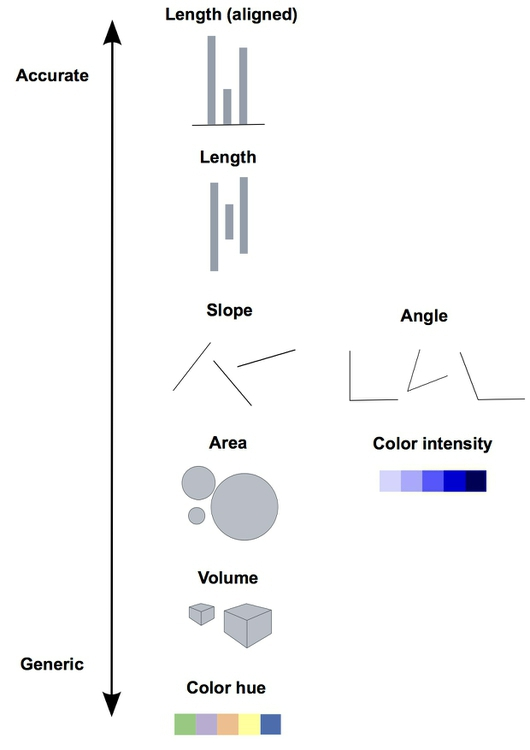
\includegraphics[width=.45\textwidth]{figure/perception}

\tiny (Figure credit: \href{https://paldhous.github.io/ucb/2016/dataviz/week2.html}{Peter Aldhous})
\end{block}

\vspace{15em}

\end{frame}


%%%%%%%%%%%%%%%%%%%%%%%%%%%%%%%%%%%%%%%%%%

\begin{frame}[fragile]{Three main types of color palettes}


\bi
  \item sequential: a gradient in one direction
  \item divergent: a gradient away from a center
  \item qualitative: categorical groupings 
\ei

\begin{block}{Setting up a small running example}

\begin{knitrout}\tiny
\definecolor{shadecolor}{rgb}{0.969, 0.969, 0.969}\color{fgcolor}\begin{kframe}
\begin{alltt}
\hlkwd{library}\hlstd{(tidyverse)}
\hlstd{gapminder} \hlkwb{<-} \hlkwd{read_csv}\hlstd{(}\hlstr{"../../data/gapminder.csv"}\hlstd{)} \hlopt
  \hlkwd{filter}\hlstd{(continent} \hlopt{==} \hlstr{"Asia"}\hlstd{)}
\end{alltt}
\end{kframe}
\end{knitrout}

\end{block}

\end{frame}


%%%%%%%%%%%%%%%%%%%%%%%%%%%%%%%%%%%%%%%%%%

\begin{frame}[fragile]{Using sequential palettes, with {\tt RColorBrewer}}

\begin{block}{Use a divergent palette to show a gradient.}
How severe? How high? Possibly an ordered grouping.

\includegraphics[width=.5\textwidth]{figure/palette-seq}

\end{block}

\end{frame}


%%%%%%%%%%%%%%%%%%%%%%%%%%%%%%%%%%%%%%%%%%

\begin{frame}[fragile]{Using sequential palettes}

Default gradient
\begin{knitrout}\tiny
\definecolor{shadecolor}{rgb}{0.969, 0.969, 0.969}\color{fgcolor}\begin{kframe}
\begin{alltt}
\hlkwd{ggplot}\hlstd{(gapminder,} \hlkwd{aes}\hlstd{(}\hlkwc{x}\hlstd{=year,} \hlkwc{y}\hlstd{=country,} \hlkwc{fill}\hlstd{=lifeExp))} \hlopt{+}
  \hlkwd{geom_tile}\hlstd{()}
\end{alltt}
\end{kframe}

{\centering 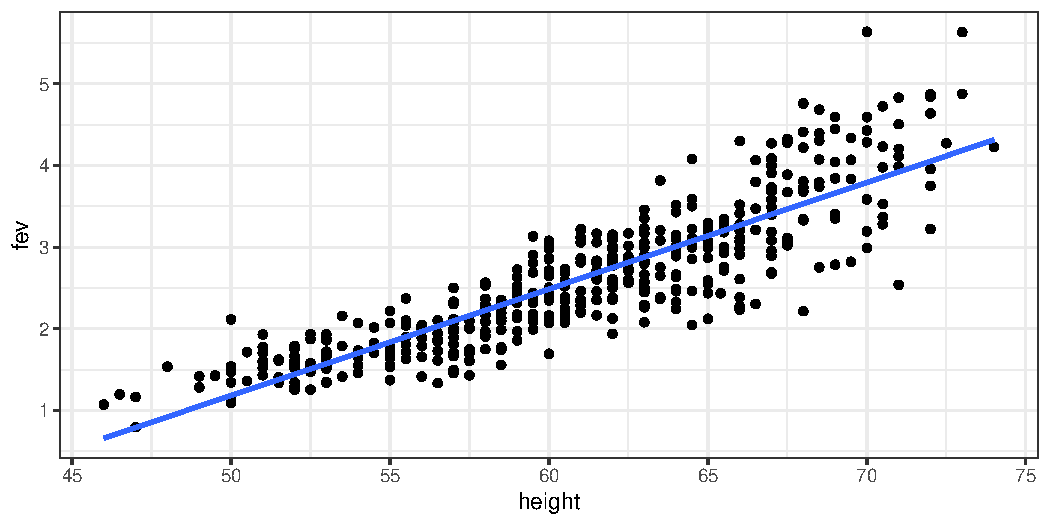
\includegraphics[width=\maxwidth]{figure/beamer-unnamed-chunk-2-1} 

}



\end{knitrout}

\end{frame}

%%%%%%%%%%%%%%%%%%%%%%%%%%%%%%%%%%%%%%%%%%

\begin{frame}[fragile]{Using sequential palettes, with assist from \href{https://colorbrewer2.org/}{colorbrewer2.org}}

Picking ColorBrewer colors.
\begin{knitrout}\tiny
\definecolor{shadecolor}{rgb}{0.969, 0.969, 0.969}\color{fgcolor}\begin{kframe}
\begin{alltt}
\hlstd{(pal} \hlkwb{<-} \hlstd{RColorBrewer}\hlopt{::}\hlkwd{brewer.pal}\hlstd{(}\hlkwc{n}\hlstd{=}\hlnum{5}\hlstd{,} \hlkwc{name}\hlstd{=}\hlstr{"Reds"}\hlstd{))}
\end{alltt}
\begin{verbatim}
## [1] "#FEE5D9" "#FCAE91" "#FB6A4A" "#DE2D26" "#A50F15"
\end{verbatim}
\begin{alltt}
\hlkwd{ggplot}\hlstd{(gapminder,} \hlkwd{aes}\hlstd{(}\hlkwc{x}\hlstd{=year,} \hlkwc{y}\hlstd{=country,} \hlkwc{fill}\hlstd{=lifeExp))} \hlopt{+}
    \hlkwd{geom_tile}\hlstd{()} \hlopt{+}
    \hlkwd{scale_fill_gradient}\hlstd{(}\hlkwc{low}\hlstd{=pal[}\hlnum{1}\hlstd{],} \hlkwc{high}\hlstd{=pal[}\hlnum{5}\hlstd{])}
\end{alltt}
\end{kframe}

{\centering 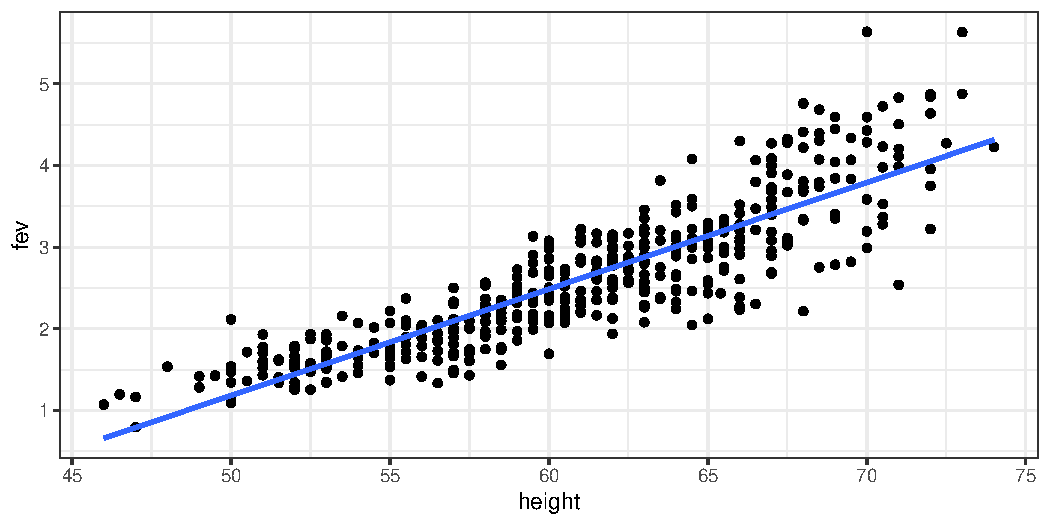
\includegraphics[width=\maxwidth]{figure/beamer-unnamed-chunk-3-1} 

}



\end{knitrout}

\end{frame}


%%%%%%%%%%%%%%%%%%%%%%%%%%%%%%%%%%%%%%%%%%

\begin{frame}[fragile]{Using qualitative palettes to show groupings\footnote{\href{https://colorbrewer2.org/}{colorbrewer2.org}}}

All palettes:\\
\includegraphics[width=.4\textwidth]{figure/palette-qual}

Only color-blind friendly ones:\\
\includegraphics[width=.4\textwidth]{figure/palette-qual-colorblind}



\end{frame}


%%%%%%%%%%%%%%%%%%%%%%%%%%%%%%%%%%%%%%%%%%

\begin{frame}[fragile]{Using qualitative palettes from {\tt RColorBrewer}}

For low-number palettes (usually less than 12 colors) you can access the palettes directly.
\begin{knitrout}\tiny
\definecolor{shadecolor}{rgb}{0.969, 0.969, 0.969}\color{fgcolor}\begin{kframe}
\begin{alltt}
\hlstd{gapminder} \hlopt
  \hlkwd{filter}\hlstd{(country} \hlopt \hlkwd{c}\hlstd{(}\hlstr{"Syria"}\hlstd{,} \hlstr{"Iraq"}\hlstd{,} \hlstr{"Iran"}\hlstd{,} \hlstr{"China"}\hlstd{,} \hlstr{"Thailand"}\hlstd{))} \hlopt
\hlkwd{ggplot}\hlstd{(}\hlkwd{aes}\hlstd{(}\hlkwc{x}\hlstd{=year,} \hlkwc{y}\hlstd{=gdpPercap,} \hlkwc{color}\hlstd{=country))} \hlopt{+}
    \hlkwd{geom_point}\hlstd{()} \hlopt{+} \hlkwd{geom_line}\hlstd{()} \hlopt{+}
    \hlkwd{scale_color_brewer}\hlstd{(}\hlkwc{type} \hlstd{=} \hlstr{"qual"}\hlstd{)}
\end{alltt}
\end{kframe}

{\centering 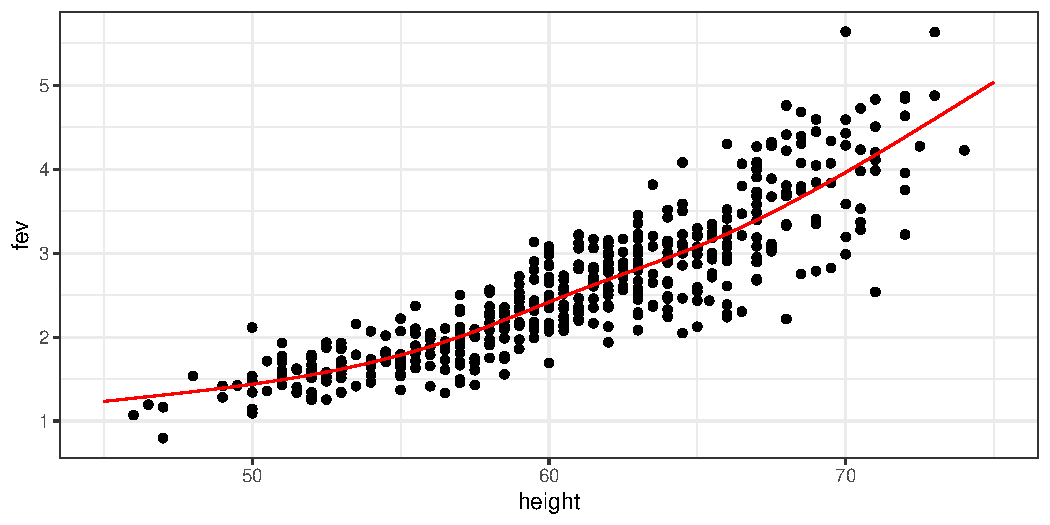
\includegraphics[width=\maxwidth]{figure/beamer-unnamed-chunk-4-1} 

}



\end{knitrout}

\end{frame}


%%%%%%%%%%%%%%%%%%%%%%%%%%%%%%%%%%%%%%%%%%

\begin{frame}[fragile]{Using divergent palettes to compare values to a reference level}

This is not a great example, because the scale is not naturally bi-directional.
\begin{knitrout}\tiny
\definecolor{shadecolor}{rgb}{0.969, 0.969, 0.969}\color{fgcolor}\begin{kframe}
\begin{alltt}
\hlstd{pal} \hlkwb{<-} \hlstd{RColorBrewer}\hlopt{::}\hlkwd{brewer.pal}\hlstd{(}\hlkwc{n}\hlstd{=}\hlnum{9}\hlstd{,} \hlkwc{name}\hlstd{=}\hlstr{"RdYlBu"}\hlstd{)}
\hlstd{(mean_lifeExp} \hlkwb{<-} \hlkwd{mean}\hlstd{(gapminder}\hlopt{$}\hlstd{lifeExp))}
\end{alltt}
\begin{verbatim}
## [1] 60.0649
\end{verbatim}
\begin{alltt}
\hlkwd{ggplot}\hlstd{(gapminder,} \hlkwd{aes}\hlstd{(}\hlkwc{x}\hlstd{=year,} \hlkwc{y}\hlstd{=country,} \hlkwc{fill}\hlstd{=lifeExp))} \hlopt{+}
    \hlkwd{geom_tile}\hlstd{()} \hlopt{+}
    \hlkwd{scale_fill_gradient2}\hlstd{(}\hlkwc{low}\hlstd{=pal[}\hlnum{1}\hlstd{],} \hlkwc{mid}\hlstd{=pal[}\hlnum{5}\hlstd{],} \hlkwc{high}\hlstd{=pal[}\hlnum{9}\hlstd{],} \hlkwc{midpoint} \hlstd{= mean_lifeExp)}
\end{alltt}
\end{kframe}

{\centering 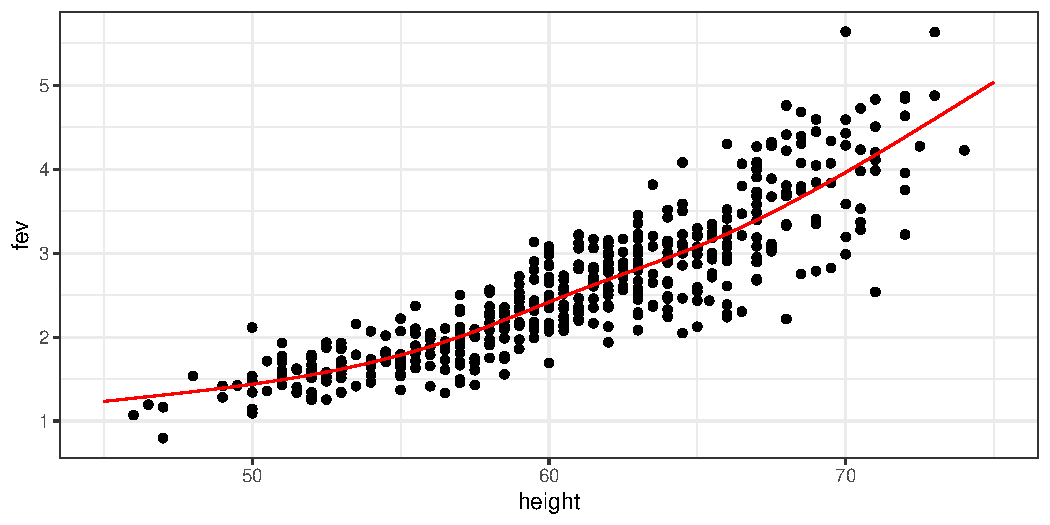
\includegraphics[width=\maxwidth]{figure/beamer-unnamed-chunk-5-1} 

}



\end{knitrout}

\end{frame}


%%%%%%%%%%%%%%%%%%%%%%%%%%%%%%%%%%%%%%%%%%

\begin{frame}[fragile]{Using divergent scale to compare model accuracy}

An example from \href{https://www.medrxiv.org/content/10.1101/2021.02.03.21250974v1}{my research}. Each cell represents the relative accuracy of the given model (column) to a baseline model for a location (row). Blue = more accurate than baseline. Red = less.

\includegraphics[width=.6\textwidth]{figure/fig-wis-location}

\end{frame}


%%%%%%%%%%%%%%%%%%%%%%%%%%%%%%%%%%%%%%%%%%

\begin{frame}[fragile]{Breakout rooms}

Consider the figure on the next slide. What visual cues do they use? Follow the note-catcher to document your observations. 

\end{frame}

%%%%%%%%%%%%%%%%%%%%%%%%%%%%%%%%%%%%%%%%%%


\begin{frame}

\centering

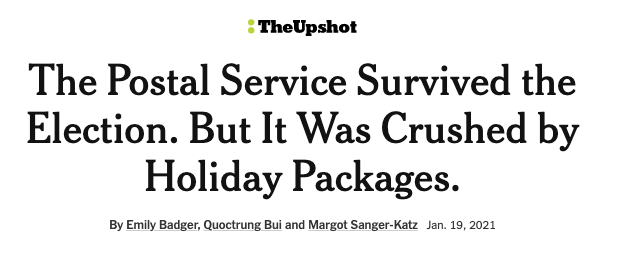
\includegraphics[width=.6\textwidth]{../lecture1-story-examples/figure-static/upshot-postal-banner.png}

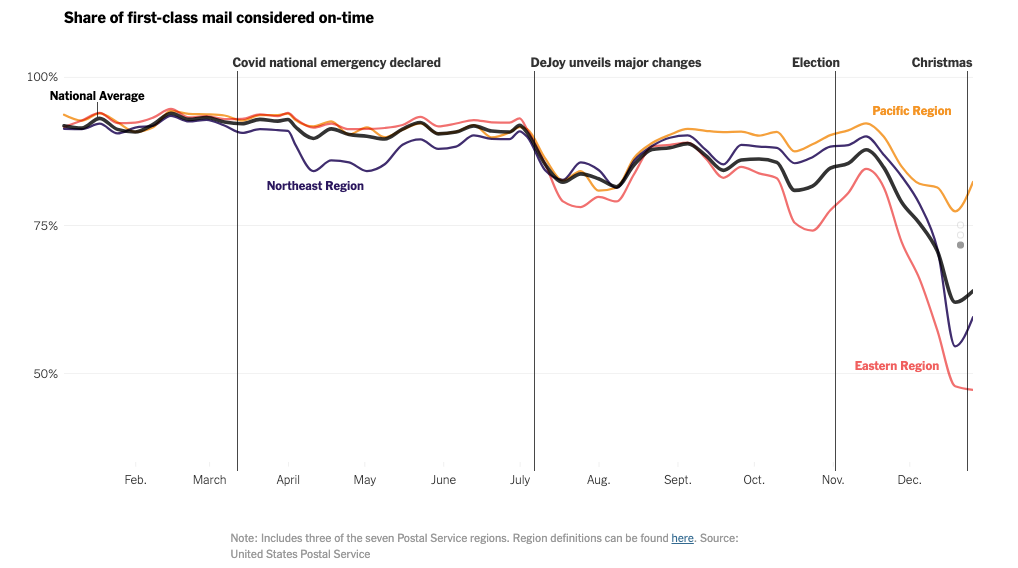
\includegraphics[width=.9\textwidth]{../lecture1-story-examples/figure-static/upshot-postal-timeseries.png}

\tiny \url{https://www.nytimes.com/interactive/2021/01/19/upshot/postal-service-survived-election-but-crushed-by-holidays.html}

\end{frame}


%%%%%%%%%%%%%%%%%%%%%%%%%%%%%%%%%%%%%%%%%%



\end{document}
